\documentclass[12pt,a4paper]{ufpr}

\usepackage[brazil]{babel}
\usepackage[utf8]{inputenc}
\usepackage{amssymb,amsmath}
\usepackage{epsfig}
\usepackage{multirow}

\usepackage{amssymb}
\usepackage{subfigure}
\usepackage{graphicx}
\usepackage{caption2}
\usepackage{setspace}
\usepackage{ps-macros}
% \usepackage{psfig}

\setcounter{secnumdepth}{3}    % n - numero de niveis de subsubsection numeradas
\setcounter{tocdepth}{3}       % coloca ate o nivel n no sumario

\title{A ser definido}
\author{Eduardo Luís Buratti}
\advisortitle{Orientador}
\advisorname{Prof. Dr. Eduardo Jaques Spinosa}
\advisorplace{Departamento de Informática, UFPR} % departamento, instituicao
\city{Curitiba}
\year{2013}

% \banca        % nao insira o nome do orientador, ja eh feito automaticamente
% {Prof. Dr. Luciano Fontoura}{Instituto de Física, USP}
% {Prof. Dr. Hélio Pedrini}{Departamento de Informática, UFPR}
% {Prof. Dr. Alexandre I. Direne}{Departamento de Informática, UFPR} % se nao houver deixe em branco {}{}
% {}{}    % se houver um quarto membro na banca, inserir nome e instituicao
% \defesa{04 de outubro de 2000} % dia em que foi realizada a defesa da dissertacao

\begin{document}

\makecapamonografia
\makerostomonografia
% \maketermo

%\singlespacing
%\onehalfspacing
\doublespacing

\pagestyle{headings}
\pagenumbering{roman}

% \chapter*{Agradecimentos}
% Agradeço primeiramente a meus pais pelo apoio e suporte que me permitiram chegar até aqui.\\

\noindent
Aos meus dois irmãos e irmã pelo exemplo e inspiração que formaram meu caráter.\\

\noindent
Ao meu professor orientador por dedicar parte de seu tempo para me guiar e motivar a cada passo deste trabalho.\\

\noindent
Aos meus amigos e colegas de trabalho pela compreensão e apoio nos momentos mais necessários.\\

\noindent
E a todos que contribuíram de forma direta ou indireta para a minha jornada, espero poder retribuir de alguma forma no futuro.

\chapter*{Resumo}
\addcontentsline{toc}{chapter}{RESUMO}
Dentre diversos seres vivos observados na natureza, destacam-se aqueles que tem capacidade de auto-organização a fim de superar os limites físicos e cognitivos individuais e então vencer obstáculos e dificuldades mais complexos de forma coletiva. Esse trabalho tem como objetivo avaliar diferentes estratégias e algoritmos para síntese de um controlador para robôs autônomos em um enxame cuja finalidade é reproduzir o comportamento coletivo de formação de caminho.\\

\noindent
Palavras-chave: Robótica de Enxame, Robótica Evolutiva, Formação de Caminho.
\newpage

\chapter*{Abstract}
\addcontentsline{toc}{chapter}{ABSTRACT}
Among several living beings observed in nature, those with self-organization capabilities stand out. In a collective way, these living beings can overcome their own physical and cognitive limitations in order to solve more complex and difficult tasks. Swarm robotics is an area of robotics concentrated into the apllication of similar concepts to solve problems in the robotics area. This work aims to evaluate several strategies and algorithms (utilizing evolutionary robotics) for synthesis of an autonomous robot controller whose purpose is to reproduce the path-formation collective behavior.\\

\noindent
Keywords: Swarm Robotics, Evolutionary Robotics, Path Formation.
\newpage

\listoffigures
\addcontentsline{toc}{chapter}{\MakeUppercase{LISTA DE FIGURAS}}
\newpage

\listoftables
\addcontentsline{toc}{chapter}{\MakeUppercase{LISTA DE TABELAS}}
\newpage

\tableofcontents

\pagenumbering{arabic}

\chapter{Introdução}
\label{introducao}

% (contexto, motivação, objetivos, estrutura)

Teste para a introdução, referência \cite{tese1}
\chapter{Robótica evolutiva}
\label{cha:evolutionary-robotics}

\section{Introdução}

Segundo Nolfi et al. \cite{nolfi1994howtoevolve}, o projeto de um controlador para robôs autônomos apresenta duas grandes dificuldades:

\begin{enumerate}
    \item A coordenação das partes de um robô é extremamente difícil, tanto a nível do sistema de controle quanto a nível mecânico. A imprevisibilidade da interação entre esses dois níveis resulta em mais dificuldades.
    \item Robôs autônomos interagem com um ambiente externo e portanto o modo como esse se comporta determina os estímulos que receberá de entrada. Essa relação introduz um efeito de longo termo difícil de prever e modelar.
\end{enumerate}

Como uma forma de automatizar esse processo, os conceitos de computação evolutiva e seus algoritmos são utilizados para a construção gradual de tais controladores. Daí, a área denominada robótica evolutiva (\textit{Evolutionary Robotics} - ER). Na literatura, Brooks \cite{brooks1992artificiallife} utiliza de programação genética para construir um programa controlador em linguagem de alto nível. Dorigo e Schenepf \cite{dorigo1993geneticsbased} tratam o problema com uso de sistemas classificadores. Hoffmann e Pfister \cite{hoffmann1996evolutionary} utilizam um controlador de lógica difusa. No entanto, a estratégia mais comum \cite{nelson2009fitness} -- e adotada nesse trabalho -- é com o uso de redes neurais artificiais \cite{cliff1992evolvingvisually} \cite{miglino1994selection} \cite{nolfi1994phenotypic}.

A Seção \ref{sec:evolutionary-computation} descreve os quatro algoritmos evolutivos avaliados nesse trabalho. A Seção \ref{sec:ann} descreve as redes neurais artificiais e, mais especificamente, o modelo utilizado para representação do controlador do robô utilizado.

\section{Computação evolutiva}
\label{sec:evolutionary-computation}

A Computação Evolutiva (CE) é uma área da computação focada em métodos de otimização global. Os algoritmos dessa área são estocásticos e utilizam metaheurísticas que, geralmente, modelam fenômenos naturais \cite{michalewicz1995heuristic}. De forma bastante abstrata, são processos que melhoram iterativamente soluções para um determinado problema a partir de um conjunto inicial geralmente aleatório.

Dentre os diversos algoritmos emergentes da computação evolutiva podemos notar alguns: algoritmo genético, programação genética, evolução diferencial, \textit{particle swarm optimization}, \textit{ant colony optimization} etc.

\subsection{Algoritmo genético}

Algoritmos genéticos (\textit{Genetic Algorithms} - GAs) são algoritmos evolutivos cuja heurística baseia-se no processo de evolução natural. Esses algoritmos codificam uma potencial solução para um problema específico em uma estrutura de dados semelhante a um cromossomo e aplica operadores de recombinação a essas estruturas a fim de preservar informação crítica \cite{whitley1994genetic}.

O algoritmo canônico inicia com uma população (geralmente aleatória) de indivíduos. Cada indivíduo representa uma possível solução ao problema e é composto de um ou mais cromossomos. Cada parâmetro da solução é codificado em um gene, ou seja, uma \textit{string} de bits. A união dos vários genes compõem um cromossomo. Em seguida, os indivíduos são avaliados em relação a qualidade desses como uma solução do problema. A função que realiza essa avaliação é chamada função de aptidão ou função de \textit{fitness}. A partir do resultado dessa avaliação, os operadores são aplicados a fim de gerar uma nova população.

\begin{algorithm}[h]
    \caption{Pseudocódigo de um algoritmo genético padrão}
    \begin{algorithmic}
        \State $P \gets $ população inicial aleatória
        \State $g \gets 0$
        \While {$g \le $ quantidade máxima de gerações}
            \State \Call{Avalia}{P}
            \State $S \gets$ \Call{Seleção}{$P$}
            \State $P \gets \varnothing$
            \ForEach {par de índividuos $(i_{1}, i_{2})$ em $S$}
                \State $P \gets P \>\> \bigcup \>$ \Call{Cruzamento}{$i_{1}, i_{2}$}
            \EndFor
            \State $P \gets $ \Call{Mutação}{$P$}
            \State $g \gets g + 1$
        \EndWhile
    \end{algorithmic}
\end{algorithm}

O operador \textbf{seleção} escolhe indivíduos para reprodução sexuada (cruzamento) ou assexuada (mutação) \cite{erik2012geneticos}.

O \textbf{cruzamento} gera novos indivíduos (\textit{offspring}) a partir da combinação de dois indivíduos selecionados, mantendo características de ambos. A taxa de cruzamento define a probabilidade de ocorrer o cruzamento entre dois indivíduos selecionados.

A \textbf{mutação} consiste na troca aleatória de alguns bits no cromossomo com probabilidade definida pela taxa de mutação.

\subsection{Algoritmos genéticos paralelos}

Algoritmos genéticos paralelos (\textit{Parallel GAs} -- PGAs) \cite{shonkwiler1993parallel} são variações dos GAs em alguns aspectos centrais aos quais a paralelização pode ser aplicada. Assim, é possível obter melhores resultados em relação a qualidade da solução e também a otimização do uso dos recursos computacionais \cite{erik2012geneticos}.

Os algoritmos genético paralelos podem ser classificados da seguinte forma \cite{cantupaz1998asurvey}:

\begin{itemize}
    \item \textbf{Mestre-escravo}: paralelização do cálculo da função de aptidão (única população).
    \item \textbf{\textit{Fine-grained}}: paralelização dos indivíduos de uma única população com frequente comunicação entre as partes.
    \item \textbf{\textit{Coarse-grained}}: diversas populações paralelas com pouca comunicação entre as partes.
\end{itemize}

Nos algoritmos genéticos paralelos \textit{coarse-grained} (\textit{Coarse-Grained Parallel Genetic Algorithms} - CGPGAs) um arquipélago é um conjunto de populações distintas denominadas ilhas e o processo de troca de indivíduos entre as ilhas é chamado migração. Dois parâmetros importantes são introduzidos: a quantidade de indivíduos que são trocados entre as ilhas (taxa de migração) e a frequência em que essas acontecem.

Outro fator importante a ser observado é a topologia dos arquipélagos, ou seja, as possibilidades de caminho para a migração entre as ilhas. Por exemplo, a Figura \ref{fig:ring} apresenta um arquipélago com topologia em anel onde cada ilha é conectada apenas com a próxima a fim de formar um ciclo. A Figura \ref{fig:barabasi-albert} mostra outro exemplo de topologia baseada no modelo Barabási-Albert \cite{albert2002statistical}.

\begin{figure}[H]
    \centering
    \begin{minipage}{.2\textwidth}
        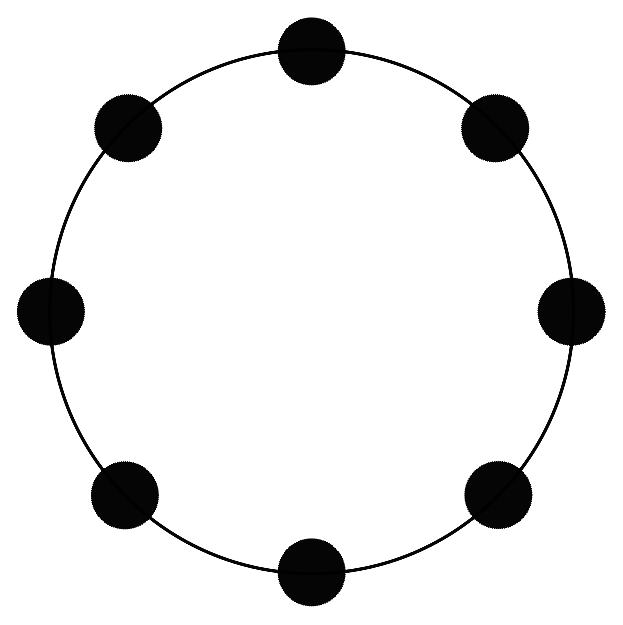
\includegraphics[width=0.9\textwidth]{figures/ring}
        \subcaption{Topologia em anel}
        \label{fig:ring}
    \end{minipage}%
    \quad\quad\quad\quad
    \begin{minipage}{.35\textwidth}
        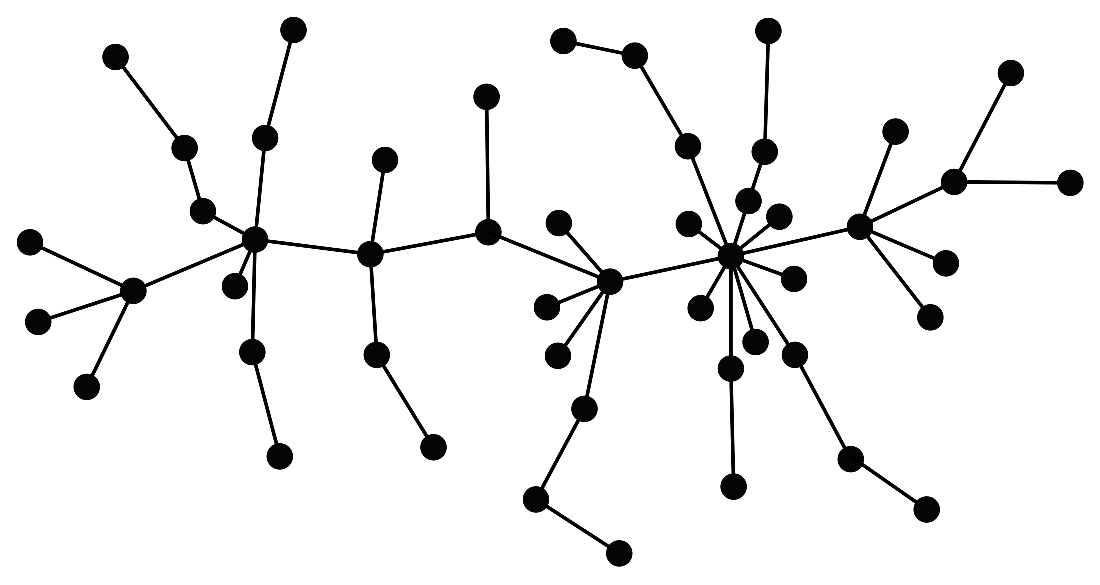
\includegraphics[width=\textwidth]{figures/barabasi-albert}
        \subcaption{Topologia baseada em redes Barabasi-Albert}
        \label{fig:barabasi-albert}
    \end{minipage}

    \caption{Exemplos de topologias de arquipélagos}
\end{figure}

\subsection{\textit{Particle Swarm Optimization}}

O método introduzido por Kennedy e Eberhart \cite{kennedy1995pso} denominado \textit{Particle Swarm Optimization} (PSO) utiliza enxames de partículas para otimização de funções não-lineares. Nesse, para a solução de um problema com $n$ parâmetros, cada partícula $i$ possuí dois vetores $n$-dimensionais: posição $x_{i} = (x_{i1}, x_{i2}, \dots, x_{in})$ e velocidade $v_{i} = (v_{i1}, v_{i2}, \dots, v_{in})$. A cada iteração $t$ ambos os vetores são atualizados da seguinte maneira:

\begin{equation}
\label{eq:pso-vel}
v_{i}^{t} = \omega v_{i}^{t-1} + \alpha \phi (p_{i}^{best} - x_{i}^{t-1}) + \beta \phi (g^{best} - x_{i}^{t-1})
\end{equation}

\begin{equation}
\label{eq:pso-pos}
x_{i}^{t} = x_{i}^{t-1} + v_{i}^{t}
\end{equation}

onde $\phi$ é um número aleatório no interalo $[0,1]$ de distribuição uniforme, $p_{i}^{best}$ é o melhor vetor posição encontrado pela partícula $i$ (localmente) e $g^{best}$ é a melhor posição encontrada por todas as partículas (globalmente).

$\omega$, $\alpha$ e $\beta$ são parâmetros do algoritmo. O parâmetro $\omega$ se traduz em um fator de inércia, ou seja, determina a dependência da velocidade em um momento em relação ao anterior. O nível de confiança nas melhores soluções encontradas localmente e globalmente são determinadas pelos parâmetros $\alpha$ e $\beta$, respectivamente.

\subsection{\textit{Discrete Particle Swarm Optimization}}

Esta variação do PSO difere na representação das partículas. No \textit{Discrete Particle Swarm Optimization} (DPSO) a posição $x_{i} = (x_{i1}, x_{i2}, \dots, x_{in})$ de uma partícula $i$ está contida num espaço discreto e cada elemento do vetor velocidade $v_{ij}$ é um vetor $m$-dimensional contendo as probabilidades de $x_{ij}$ assumir cada um dos $m$ possíveis valores discretos.

Matematicamente,

\noindent\begin{minipage}{.5\linewidth}
$$
P(x_{i,j} = k) = \frac{\sigma (v_{i,j,k})}{S_{i,j}}
$$
\end{minipage}%
\begin{minipage}{.5\linewidth}
$$
S_{i,j} = \sum_{k}^{m} \sigma(v_{i,j,k})
$$
\end{minipage}\\

onde $\sigma$ é a função \textit{sigmoid}, $v$ é o vetor de velocidades e $x$ é o vetor posição.

Desse modo, a probabilidade de $x_{i,j}$ assumir o valor $k$ é determinada pela velocidade $v_{i,j,k}$. Note que $S_{i,j}$ é um coeficiente de normalização e tem a finalidade de permitir que $x_{i,j}$ possa assumir qualquer valor $k$.


\section{Redes neurais artificiais}
\label{sec:ann}

Redes neurais artificias (RNAs) são sistemas computacionais inspirados em sistemas nervosos animais capazes de aprendizado. Matematicamente, RNAs são aproximadores universais \cite{hornik1989universal}. Um RNA é composto por uma rede de unidades de processamento simples (neurônios) que possuem um sinal de saída e podem receber um ou mais sinais de entrada.

\subsection{\textit{Multi-Layer Perceptron}}

Uma rede neural \textit{Multi-Layer Perceptron} (MLP) é composta por uma série de neurônios organizados em camadas, onde cada neurônio recebe, como entrada, a saída dos neurônios da camada anterior. Uma rede com uma camada intermediária é capaz de aproximar qualquer função contínua. Com duas camadas intermediárias, qualquer função pode ser aproximada \cite{cybenko1989mlp}.

\begin{figure}[H]
    \centering
    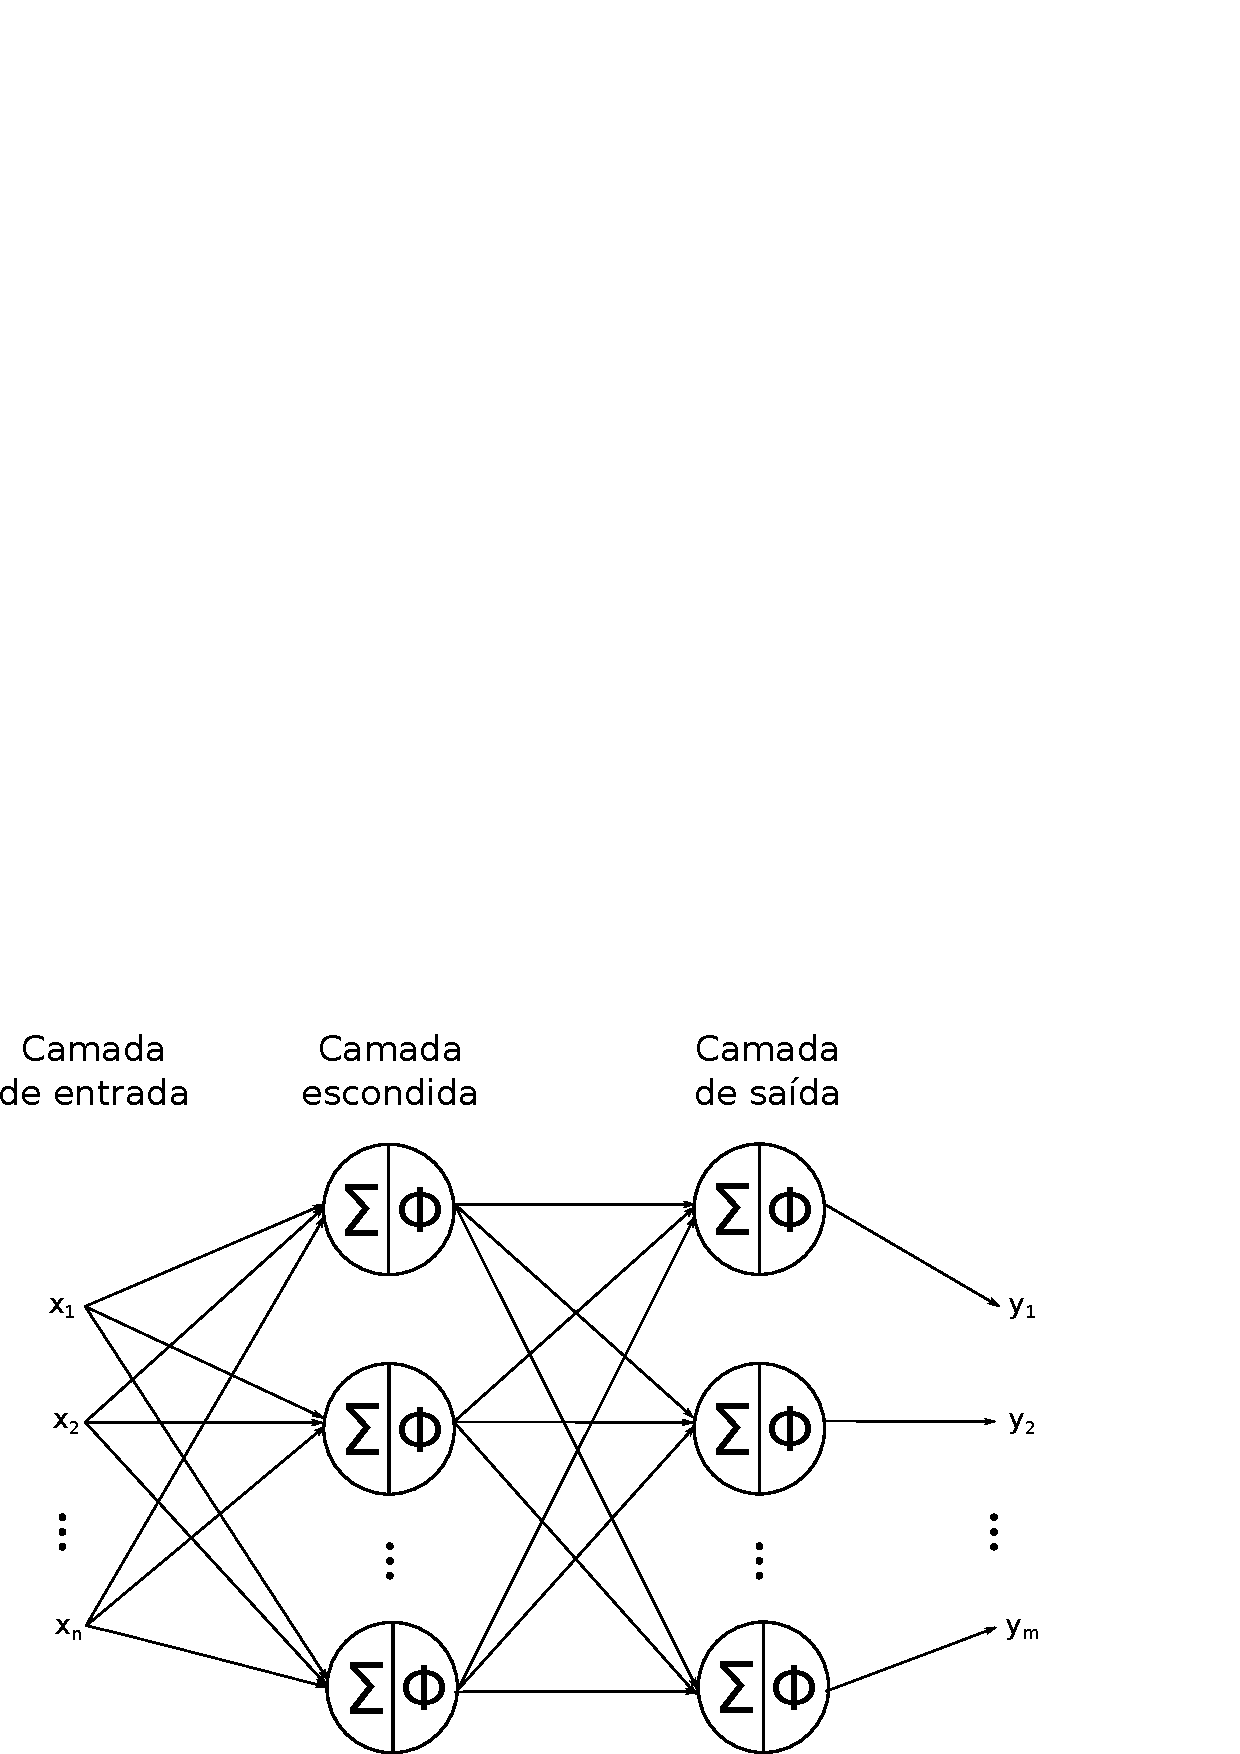
\includegraphics[width=0.5\textwidth]{figures/mlp}
    \caption{Multi-layer Perceptron}
    \label{fig:mlp}
\end{figure}

A saída (y) de um neurônio é determinada pela aplicação de uma função de ativação \(\sigma\) sobre a combinação linear ponderada de todas as suas \(n\) entradas \((x_1, x_2, \dots , x_n)\).

Matematicamente,

\[ y = \sigma ( \sum_{i=1}^{n} w_i x_i ) \]

onde \(w_i\) é um peso associado a entrada \(i\).

Diversas funções pode assumir o papel de função de ativação, sendo as mais comuns:
a função degrau (\ref{eq:degrau}) e a função sigmóide (\ref{eq:sigmoid}).

\begin{equation} \label{eq:degrau}
    \sigma (x) = \left\{
    \begin{array}{l l}
        0 & \quad \text{se } x < 0\\
        1 & \quad \text{caso contrário}
    \end{array} \right.
\end{equation}

\begin{equation} \label{eq:sigmoid}
    \sigma (x) = \frac{1}{1 + e^{-x}}
\end{equation}

É comum encontrar, em cada uma das camadas, um neurônio adicional cuja entrada é sempre \(1\). Este neurônio especial tem o nome de \textit{bias} e a finalidade de deslocar a função de ativação para direita ou esquerda.

O ajuste dos pesos \((w_1, w_2, \dots , w_n)\) é chamado treinamento e existe em duas formas:

\begin{description}
    \item[Supervisionado]: É fornecido ao algoritmo um conjunto de treinamento composto de entradas e suas respectivas saídas. O algoritmo iterativamente ajusta os pesos da rede a fim de que, para cada entrada do conjunto de treinamento, a saída da rede aproximem-se da saída esperada.
    \item[Não supervisionado]: Não demanda conjunto de treinamento, os pesos são ajustados considerando a aptidão da rede à solução do problema.
\end{description}

\subsection{\textit{Time-Delay Neural Network}}
\label{sec:tdnn}

Estendendo os conceitos das redes MLP, uma \textit{Time-Delay Neural Network} (TDNN) permite à cada neurônio armazenar um histórico dos sinais de entrada (Figura \ref{fig:tdnn}). Isto permite que a rede ganhe sensibilidade à padrões temporais, ou seja, a rede pode adaptar-se não só a simples padrões como também a sequências de padrões \cite{kaiser1994tdnn}.

\begin{figure}[H]
    \centering
    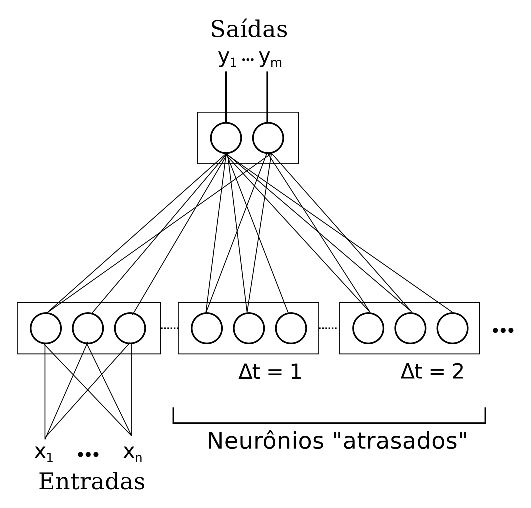
\includegraphics[width=0.5\textwidth]{figures/tdnn}
    \caption{Time-Delay Neural Network}
    \label{fig:tdnn}
\end{figure}
\chapter{Robótica de enxame}
\label{swarm}

\section{Introdução}

Observando os seres vivos presentes na natureza, podemos facilmente extrair algumas qualidades que estes apresentam: flexibilidade, robustez, descentralização, auto-organização. Em grande parte, o motivo por trás dessas qualidades é a coletividade. Por exemplo, em colônias de insetos sociais, diversos indivíduos se auto-organizam para realizar tarefas cuja  escala e complexidade superam, e muito, os limites físicos e cognitivos de cada indivíduo \cite{navarro2012introduction}. Podemos visualizar uma colônia como um único super-organismo \cite{trianni2011swarm} e podemos interpretar inteligência como uma característica que emerge das interações entre componentes simples e interdependentes de um sistema.

Sob esse ponto de vista, uma série de algoritmos computacionais têm sido propostos em uma área de pesquisa denominada inteligência coletiva (\textit{swarm intelligence}) \cite{bonabeau1999swarm} \cite{kennedy2001swarm}. Da mesma forma, a área denominada robótica de enxame (\textit{swarm robotics}) estuda como grupos de agentes relativamente simples podem ser projetados a fim de resultar em um determinado comportamento coletivo a partir de interações entre os próprios agentes e os agentes e o ambiente \cite{sahin2005swarm}.

\section{Comportamentos coletivos}

Na literatura da área encontram-se diversos comportamentos coletivos a serem reproduzidos no contexto da robótica. Alguns relativamente simples e outros bastante mais complexos, que em geral dependem da execução coordenada de alguns dos comportamentos coletivos simples.

O comportamento de \textbf{agregação}, por exemplo, consiste simplesmente na reunião dos robôs do enxame e é utilizado por outros comportamentos complexos, como o movimento coletivo, a auto-montagem e a formação de padrões, nos quais em determinados momentos o enxame se reúne.

No comportamento de \textbf{dispersão}, o enxame se distribui de modo a ocupar a maior área possível do espaço sem perder comunicação. É útil em tarefas que envolvam a exploração coletiva de um território desconhecido.

A \textbf{formação de padrões} é um comportamento em que os robôs devem movimentar-se de maneira coordenada para distribuírem-se no espaço segundo um determinado modelo de posicionamento.

Já no comportamento de \textbf{movimento coletivo} o enxame deve mover-se em conjunto e de maneira coesa \cite{sperati2008evolving}. Há, nesse caso, uma clara inspiração na natureza, por exemplo na maneira como se movimentam pássaros em um bando ou peixes em um cardume. Pelo menos dois tipos de movimento coletivo podem ser identificados: \textbf{formation}, em que o posicionamento e a orientação dos robôs mantêm-se fixa, e \textbf{flocking}, em que isso não acontece.

O comportamento de busca por alimento (\textbf{foraging}) observado na natureza pode inspirar uma gama mais ampla de problemas em que os robôs devem encontrar as coordenadas de um ponto do ambiente com características definidas.

A \textbf{formação de caminho} é uma variação de movimento coletivo que também se enquadra em busca por alimento. Visa o trajeto do enxame pelo menor caminho entre dois pontos, assim como, na natureza, as formigas utlizam de feromônios para encontrar e navegar pelo menor caminho entre o formigueiro e alguma fonte de alimento.

\textbf{Alocação de tarefas} é um comportamento genérico que se aplica a diversos problemas em que o enxame precisa, de maneira coletiva e descentralizada, definir a tarefa que cabe a cada robô. Trata-se de um problema relativamente complexo em que diversos estudos vêm sendo realizados.

O \textbf{transporte coletivo} de objetos é outro comportamento facilmente observável na natureza também em colônias de formigas. Envolve alto grau de coordenação e depende de vários dos comportamentos básicos mais simples \cite{gross2006autonomous}.

Um comportamento com importante aplicação na exploração de ambientes desconhecidos é o do \textbf{mapeamento coletivo}, em que o comportamento de dispersão é associado à troca de informações entre robôs com o objetivo de produzir uma representação mais ampla do ambiente.

Outro comportamento relativamente complexo é a \textbf{auto-montagem} \cite{christensen2007mechanism}, que consiste na agregação e interconexão de robôs formando padrões que podem ser posteriormente utilizados para a solução coletiva de problemas.

\section{Formação de caminho}

Da observação do comportamento de diversas espécies de formigas, nota-se o uso de químicos (feromônios) para estabelecer uma forma de comunicação que permite: o recrutamento em massa de indivíduos e a formação dinâmica de um caminho para transporte do alimento para dentro da colônia.

No contexto de robótica de enxame, Fujisawa et al. \cite{fujisawa2008pheromone} recria com sucesso esse comportamento em um grupo de robôs. No entanto, a síntese, armazenamento, fator de evaporação e detecção confiável dos quimícos não é nada simples e dificulta o uso prático de tal método.
Por outro lado, diversas abordagens ao problema procuram alternativas aos feromônios, por exemplo: projeção luminosa \cite{garnier2007alice}, \textit{RFID}\footnote{\textit{Radio-frequency identification -- Identificação por radiofrequência.}} \cite{mamei2007rfid}, trilhas virtuais \cite{payton2001pheromone} etc.

Neste trabalho focaremos no seguinte problema: recriar o comportamento de formação de caminho de forma eficiente -- entende-se menor caminho -- entre duas áreas alvo por um enxame de robôs. A posição de cada área alvo é aleatória e desconhecida pelos robôs. A Figura \ref{fig:path-formation} apresenta um exemplo de instância do problema.

\begin{figure}[H]
    \centering
    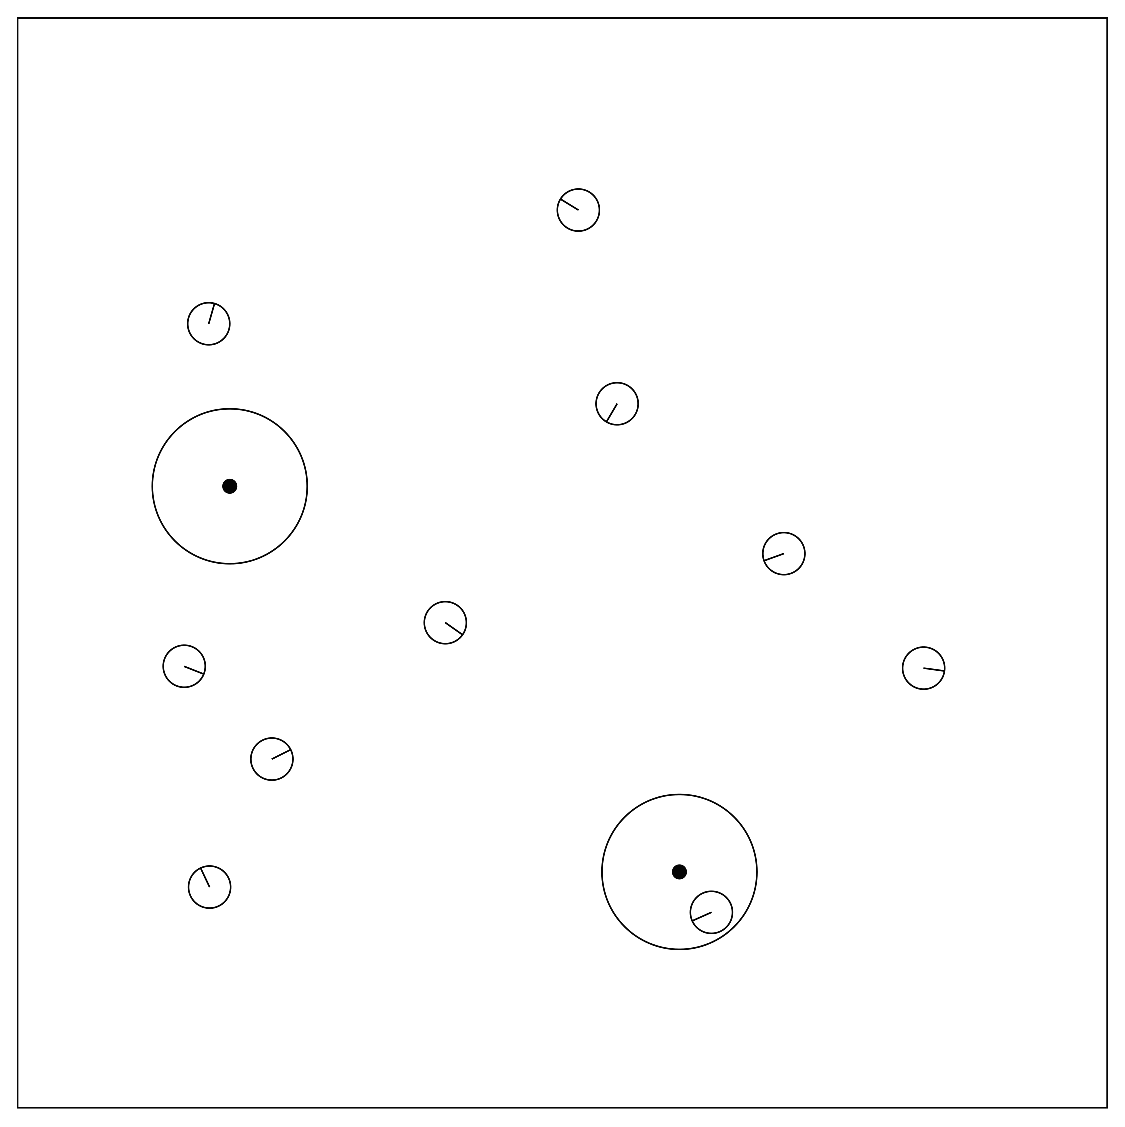
\includegraphics[width=0.5\textwidth]{figures/path-formation}

    \caption{Exemplo de instância do problema de formação de caminho com 10 robôs. As duas circunferências maiores representam as áreas alvo e as menores representam os robôs.}
    \label{fig:path-formation}
\end{figure}
\chapter{Implementação}
\label{implementacao}

\section{Introdução}

\section{Ambiente de simulação}

Os algoritmos de otimização utilizados na fase de treinamento (seção \ref{optimization-algorithms}) necessitam de múltiplas avaliações da função de \textit{fitness} (na ordem das dezenas de milhar). Conforme mencionado anteriormente (), a avaliação da função de \textit{fitness} consiste na observação do movimento dos robôs por um determinado intervalo de tempo. Logo, a utilização de robôs reais em um ambiente físico é, apesar de possível, impraticável visto o tempo demandado por tal método. Além disso, não temos a disposição o número necessário de robôs para a realização dos experimentos.

Assim, surge naturalmente a necessidade de um ambiente de simulação virtual que imite com fidelidade os robôs e o ambiente à que estes serão submetidos. A forma mais comum de simulação baseia-se na aplicação de mecânica Newtoniana, porém Miglino et al. \cite{miglino96evolving} aponta algumas dificuldades que podem ser encontradas com este tipo de simulador na fase de treinamento:
\begin{enumerate}
    \item Vários simuladores não consideram todas as leis da física envolvidas na interação entre agentes reais com o ambiente, por exemplo massa, peso, fricção, inércia etc.
    \item Sensores físicos retornam valores incertos e comandos enviados aos atuadores têm efeitos incertos. Em contraste, os ambientes de simulação geralmente retornam informações perfeitas.
    \item Diferentes sensores e atuadores, mesmo que aparentemente idênticos, podem apresentar pequenas mudanças mecânicas ou elétricas levando a diferentes comportamentos. Este fato é geralmente ignorado em simuladores.
\end{enumerate}

Estas dificuldades podem impedir a transição entre o ambiente de treinamento e o ambiente real.

Em seguida, Miglino et al. \cite{miglino96evolving} propõe um modelo de simulação baseado em amostragem. Utilizando um robô no ambiente real, constrói-se uma tabela contendo amostragens do deslocamento linear e angular para diferentes valores aplicados aos atuadores. A partir daí, as fórmulas de física clássica do simulador são substituídas por consultas nesta tabela. De forma análoga, os sensores do robô são amostrados para cada uma das diferentes classes de obstáculos presentes no ambiente.

% Implementação
% - Introdução
% - Simulação (box2d, atual)
% - Execução em paralelo (OpenCL)
% - Ferramenta para acompanhamento de experimentos
\chapter{Experimentos}
\label{experimentos}

\section{Introdução}

Dividimos os experimentos em duas partes: algoritmos de treinamento e cenários de treinamento. Na primeira, realizamos comparações entre quatro algoritmos de treinamento (GA, CGPGA, PSO, DPSO) a fim de escolher o mais apto a produzir bons resultados. Em seguida, fazemos um estudo sobre cinco diferentes cenários de treinamento e o efeito de cada para resolução do problema de formação de caminho.

\section{Algoritmos de treinamento}

Antes de mais nada, é necessário determinar como será feita a representação dos parâmetros da rede neural. No PSO, uma solução é representada por um vetor de valores contínuos (vetor posição), nesse caso a representação é direta e cada elemento do vetor equivale á um parâmetro (um peso, \textit{bias} ou \textit{time constraint}).

Os outros três algoritmos representam soluções como valores discretos, portanto os parâmetros são discretizados, uniformemente, em 256 valores.

No caso do GA e do CGPGA, estes valores discretos são concatenados formando uma string de bits.

\subsection{GA}

O algoritmo inicia com uma uma população de 120 indivíduos gerados aleatoriamente e executa por 500 gerações. A cada geração 20 indivíduos são selecionados pelo método da roleta russa e aplicam os operadores de cruzamento e mutação gerando uma nova população (cada indivíduo selecionado gera 6 novos indivíduos). Os seis melhores indivíduos são mantidos na nova população (elitismo). A estrategia de cruzamento é a de ponto único e ocorre a uma taxa de 70\%. A inversão de cada um dos \textit{bits} dos cromossomos acontece com 3\% probabilidade (mutação).

\subsection{CGPGA}

O experimento com CPGA utiliza quatro ilhas em anel, cada uma com uma população de 30 indivíduos. Os parâmetros são iguais aos descritos na seção anterior, com exceção do elitismo (que nesse caso é de 3 indivíduos) e da quantidade de indivíduos selecionados (5 indivíduos).

\subsection{PSO}

Assim como no GA, a população de partículas é iniciado com 120 indivíduos e executa 500 iterações. O vetor velocidade $v_{i} = (v_{i,1}, v_{i,2}, \dots, v_{i,n})$ e o vetor posição $x_{i} = (x_{i,1}, x_{i,2}, \dots, x_{i,n})$ da partícula $i$ a cada iteração $t$ é atualizada da seguinte forma:

\begin{equation}
v_{i}^{t} = \omega v_{i}^{t-1} + \alpha \phi (p_{i}^{best} - x_{i}^{t-1}) + \beta \phi (g^{best} - x_{i}^{t-1})
\end{equation}

\begin{equation}
x_{i}^{t} = x_{i}^{t-1} + v_{i}^{t}
\end{equation}

onde $\phi$ é um número aleatório de distribuição uniforme [0,1], $p_{i}^{best}$ é melhor vetor posição encontrado pela partícula $i$ e $g^{best}$ é a melhor posição encontrada por todas as partículas.

Os parâmetros $\omega$, $\alpha$ e $\beta$ escolhidos para os experimentos são 0.9, 2.0 e 2.0, respectivamente.

\subsection{DPSO}

Esta variação do PSO utiliza os mesmo parâmetros de tal, a diferença está na representação da posição e velocidade das partículas. No DPSO, o vetor posição $x_{i} = (x_{i1}, x_{i2}, \dots, x_{in})$ de uma partícula $i$ está contido num espaço $n$-dimensional discreto e o vetor velocidade $v_{i} = (v_{i,1,1}, v_{i,1,2}, \dots, v_{i,n,m})$ contém as probabilidades da partícula assumir determinadas posições. Ou seja,

$$
S_{i,j} = \sum_{k}^{m} \sigma(v_{i,j,k})
$$

$$
P(x_{i,j} = k) = \frac{\sigma (v_{i,j,k})}{S_{i,j}}
$$

onde $\sigma$ é a função \textit{sigmoid}, $v$ é o vetor de velocidades e $x$ é o vetor posição. Desse modo, a probabilidade de $x_{i,j}$ assumir um valor $k$ é determinada pela velocidade $v_{i,j,k}$.

Note que $S_{i,j}$ é um coeficiente de normalização e tem a finalidade de permitir que $x_{i,j}$ possa assumir qualquer valor de $k$.

\section{Cenários de treinamento}

Na Seção \ref{sec:training}, vimos a definição da função de \textit{fitness} e como é feito o treinamento. A cada geração (ou iteração) do algoritmo de treinamento, todos os indivíduos (ou partículas) são testados no simulador por um intervalo de tempo $T$ = 10 minutos ($T_{A}$ = 1 minuto e $T_{B}$ = 9 minutos). Porém, devido a aleatoriedade das posições inicias de cada robô e áreas alvo em cada teste, o resultado (\textit{fitness}) de uma única avaliação pode não ser representativo da aptidão daquele indivíduo. Por esse motivo, a \textit{fitness} de um indivíduo é dada pela média de \textit{fitness} de vários testes com configurações específicas. O conjunto desses vários testes define um cenário de treinamento.

O primeiro cenário avaliado ($c_{1}$) consiste de 16 testes onde, em cada um, a posição inicial das áreas alvo é aleatória, porém a distância, em centímetros, entre elas está no intervalo [80..140], obrigatoriamente.

(definir cenários $c_{2}$ $c_{3}$ e $c_{4}$)

Em todos os cenários, a posição dos robôs é aleatória para cada teste.
\chapter{Resultados}
\label{resultados}

\begin{figure}[h]
    \centering
    \begin{minipage}{.4\textwidth}
        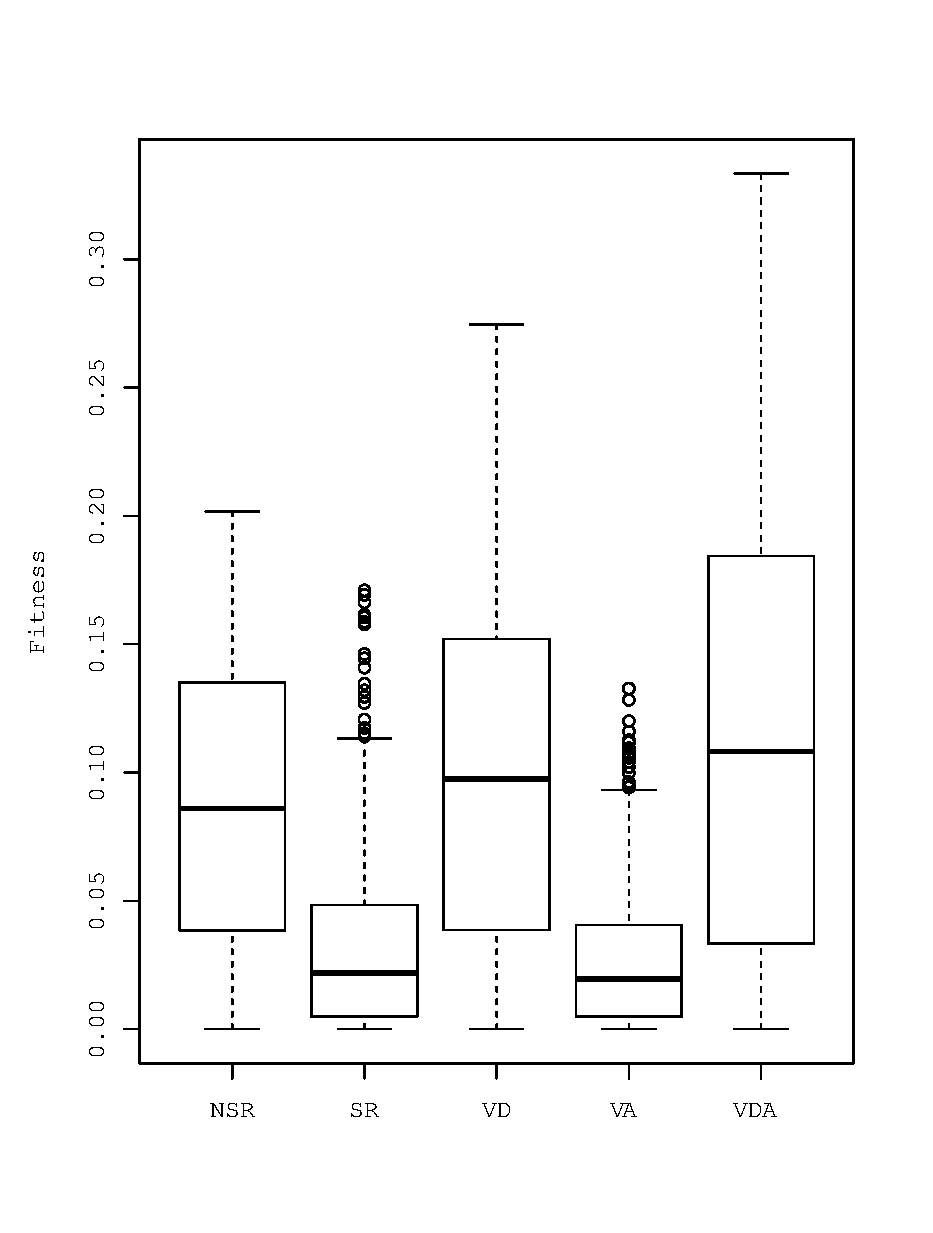
\includegraphics[width=\textwidth]{figures/reeval-nsr}
        \subcaption{NSR}
        \label{fig:reeval-nsr}
    \end{minipage}%
    \quad
    \begin{minipage}{.4\textwidth}
        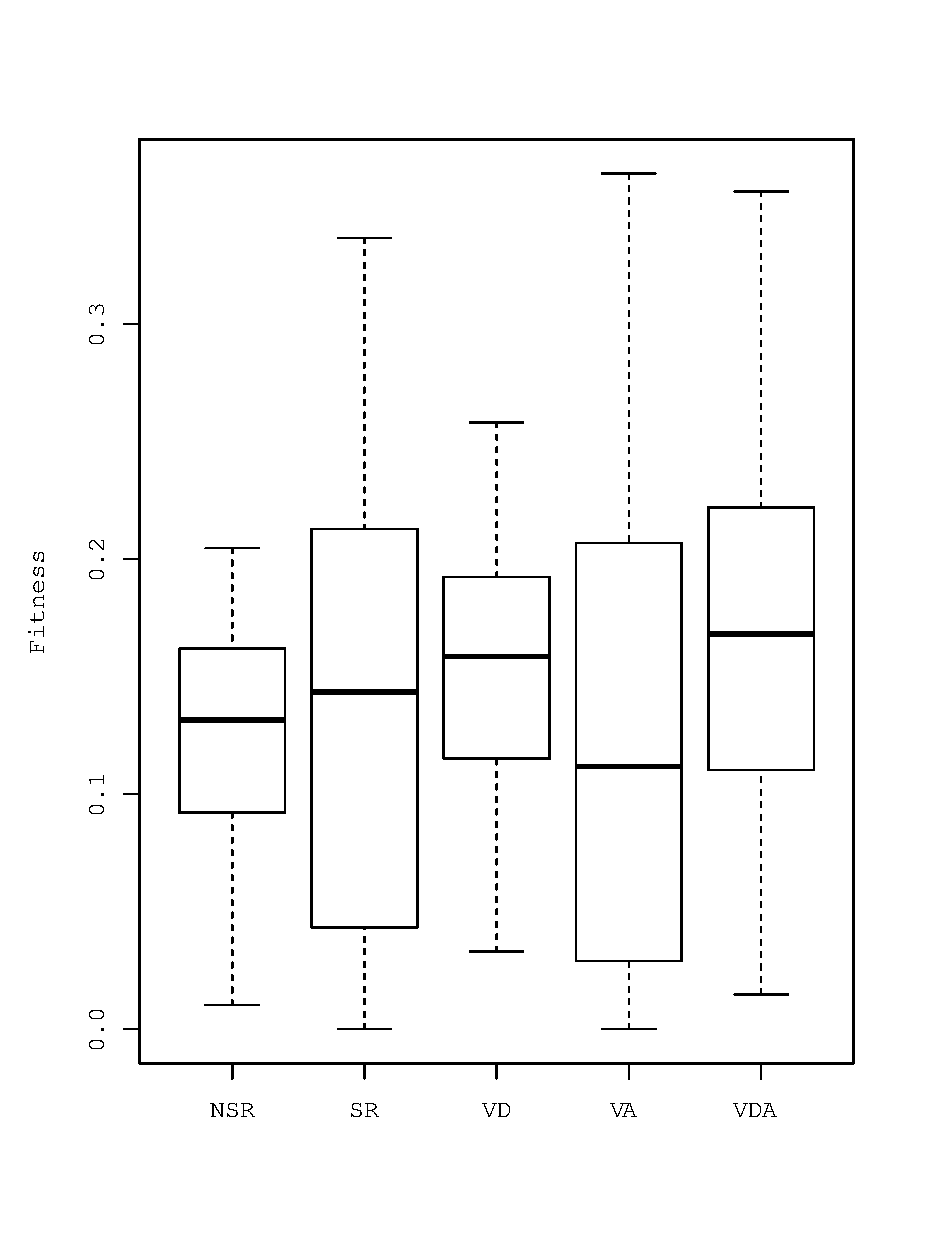
\includegraphics[width=\textwidth]{figures/reeval-sr}
        \subcaption{SR}
        \label{fig:reeval-sr}
    \end{minipage}

    \caption{Reavaliações}
\end{figure}

\begin{figure}[h]
    \centering
    \begin{minipage}{.5\textwidth}
        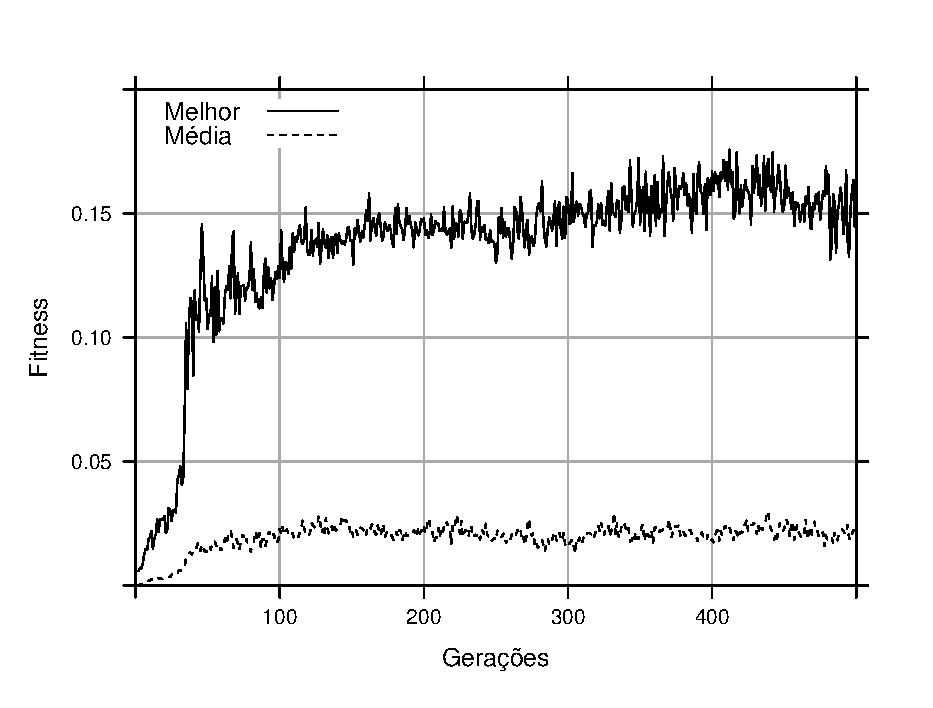
\includegraphics[width=\textwidth]{figures/fitness-GA}
        \subcaption{GA}
    \end{minipage}%
    \begin{minipage}{.5\textwidth}
        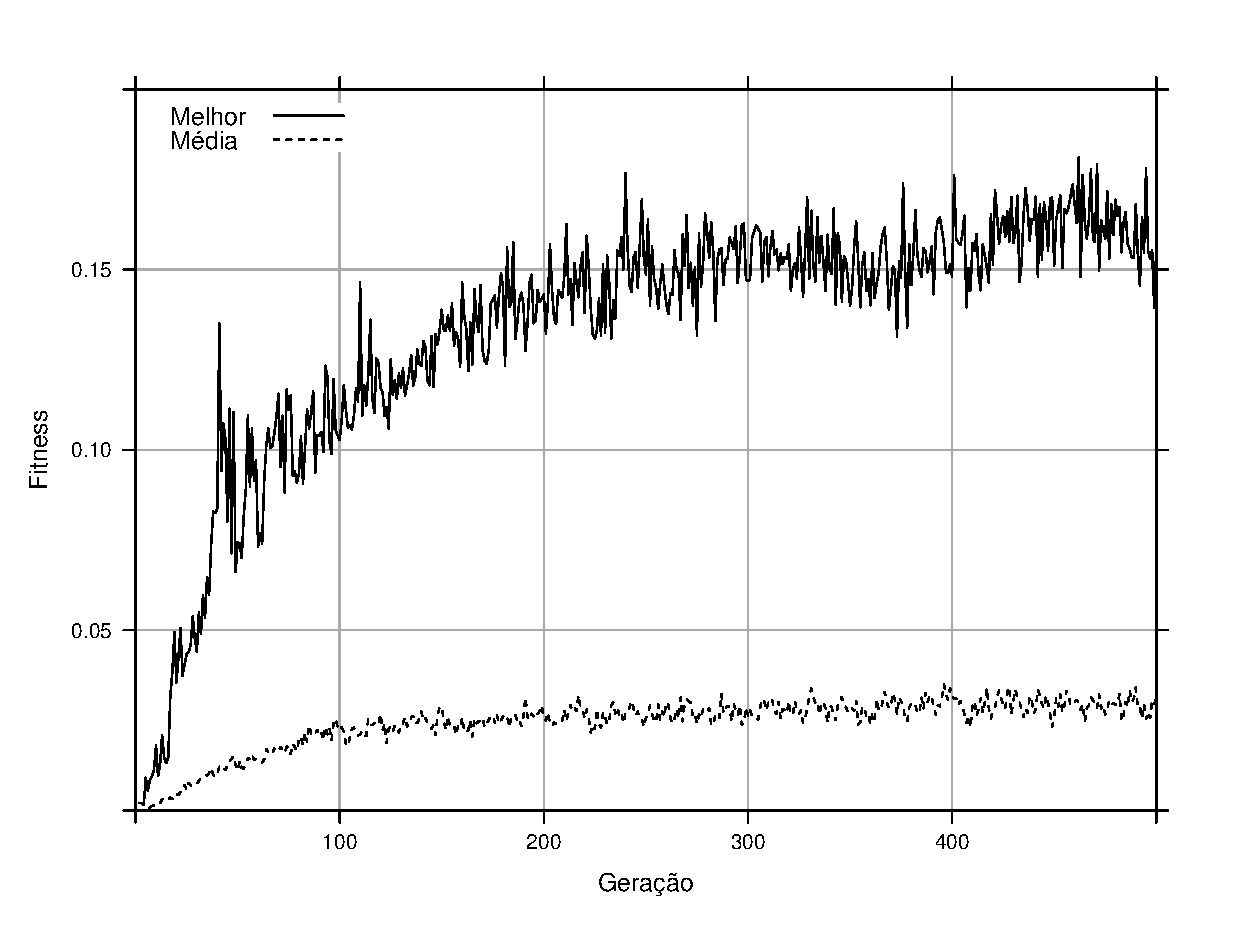
\includegraphics[width=\textwidth]{figures/fitness-PGA}
        \subcaption{CGPGA}
    \end{minipage}

    \begin{minipage}{.5\textwidth}
        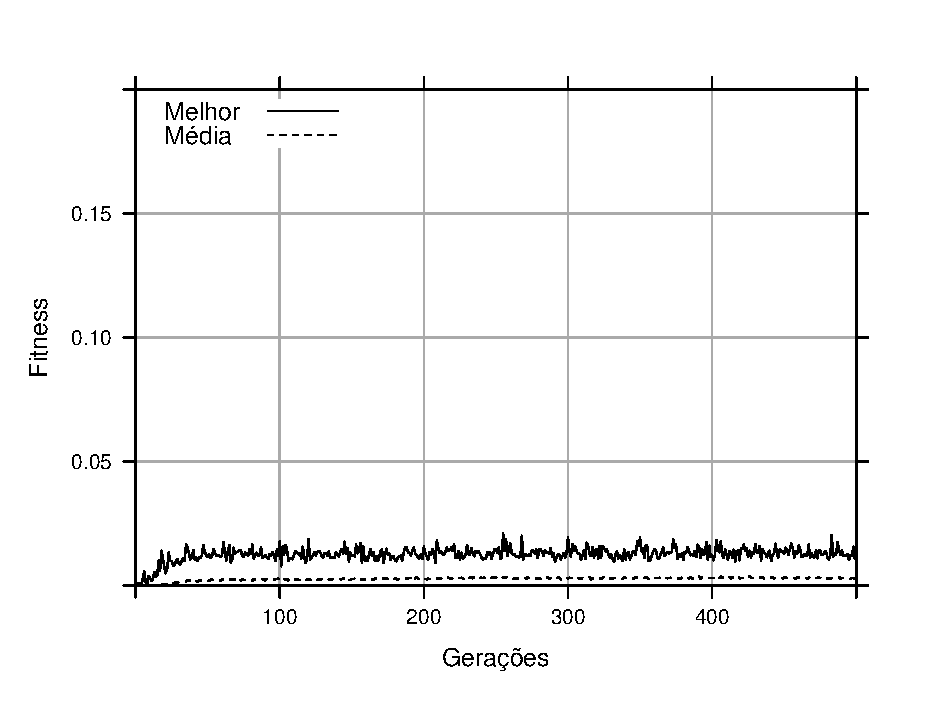
\includegraphics[width=\textwidth]{figures/fitness-PSO}
        \subcaption{PSO}
    \end{minipage}%
    \begin{minipage}{.5\textwidth}
        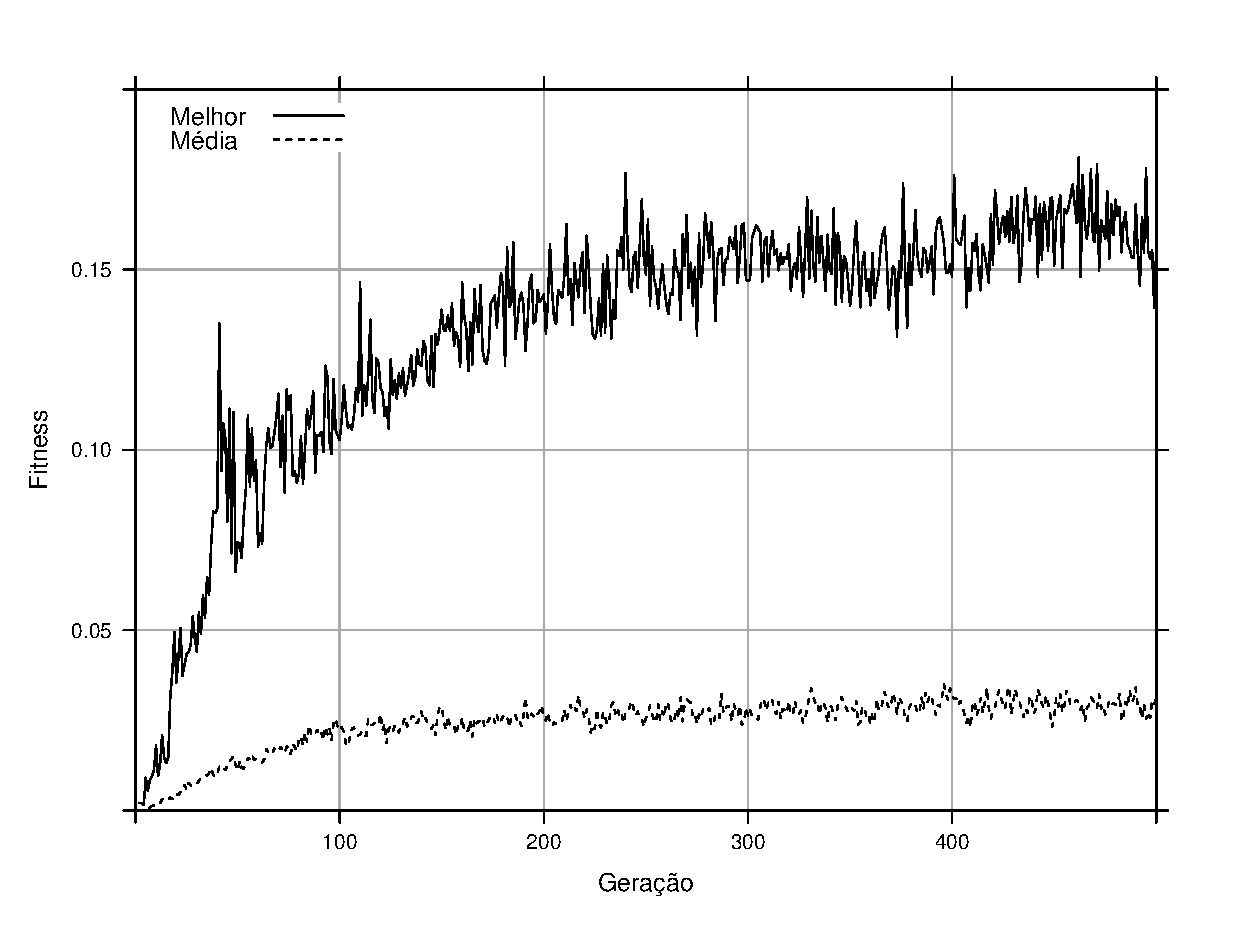
\includegraphics[width=\textwidth]{figures/fitness-PGA}
        \subcaption{DPSO}
    \end{minipage}

    \caption{Fitness}
\end{figure}
\chapter{Conclusão}
\label{cha:conclusion}

Este trabalho apresentou uma abordagem que parte da robótica evolutiva para reproduzir o comportamento de formação de caminho no contexto da robótica de enxame. Um simulador e alguns algoritmos de treinamento foram implementados para estudo e análise de diversas estratégias na tentativa de aprimorar as soluções encontradas para a execução de tal comportamento coletivo.

Para melhor utilização dos recursos computacionais disponíveis, o simulador foi desenvolvido utilizando a plataforma \textit{OpenCL}, permitindo a execução paralela em CPUs e GPUs, o que resultou em uma redução considerável no tempo necessário para cada experimento. De outra forma não seria possível realizar a análise experimental deste trabalho em tempo hábil.

A partir da análise dos resultados, verificou-se que o não determinismo da função de \fitness degrada o desempenho de um algoritmo evolutivo. Assim, na fase de treinamento, a transformação dessa função a fim de reduzir fatores aleatórios -- e aproximá-la de uma função determinística -- de fato resulta em melhor desempenho. No entanto, deve ser feita com cuidado visto que o treinamento pode explorar alguma característica exposta pela transformação que não estará presente no ambiente real.

Dentre os algoritmos de treinamento estudados (GA, CGPGA, PSO e DPSO), o GA com elitismo apresentou o melhor resultado. Para esse problema, a modelagem em ilhas do CGPGA não contribuiu na evolução da solução.

Em trabalhos futuros, cabe uma análise do PSO com outras topologias de vizinhança e/ou estratégias para evitar convergência prematura. Além disso, outros modelos de redes neurais podem ser implementados com o objetivo de permitir que o enxame execute tarefas mais complexas. Dentre elas, destacam-se as redes neurais auto-organizáveis.

\bibliographystyle{brazil}
\bibliography{referencias}
% utilize macros (3 primeiras letras do mes em ingles, minusculas) no seu
% .bib para atribuir o nome do mes em portugues nas referencia,
% se o style for brazil, outros estilos tambem aceitam estas macros
% Ex:
%
% @InProceedings{teste,
%   author =       {Luciano}
%   year =         {2000}
%   month =        {}#sep;
% }

\addcontentsline{toc}{chapter}{BIBLIOGRAFIA}

\end{document}